%%
% The BIThesis Template for Graduate Thesis
%
% Copyright 2020-2023 Yang Yating, BITNP
%
% This work may be distributed and/or modified under the
% conditions of the LaTeX Project Public License, either version 1.3
% of this license or (at your option) any later version.
% The latest version of this license is in
%   https://www.latex-project.org/lppl.txt
% and version 1.3 or later is part of all distributions of LaTeX
% version 2005/12/01 or later.
%
% This work has the LPPL maintenance status `maintained'.
%
% The Current Maintainer of this work is Feng Kaiyu.
%
% Compile with: xelatex -> biber -> xelatex -> xelatex

\chapter{Experiment Evaluation}

This chapter evaluates the adversarial malware sample generation method based on RL. First, hardware and software configurations in this experiment and evaluation metrics are introduced. Second, the experimental results are presented, including comparative experiments for each module to verify its reliability. Finally, the proposed model is compared with other models addressing similar tasks in academia.

\section{Experimental Environment Configuration}

Experiments in this research were conducted on a host configured with a 64-bit Linux operating system. RL environments were used to train malware samples and generate adversarial samples. The experimental platform utilized a custom environment based on gym-malware to simulate real software behavioral characteristics. To enhance training efficiency and flexibility, the ChainerRL and PyTorch frameworks were jointly employed. For model construction, the ACER and PPO algorithm modules from ChainerRL were used to jointly optimize the agent's policy and value networks. Sample interactions in the environment were managed via gym-malware's interface, which encapsulates action spaces and state transition functionality. To increase sample diversity, the training process uses the EpisodicReplayBuffer to store historical interaction trajectories and introduces a time-step reward decay mechanism. Detailed experimental environment specifications are shown in Table \ref{tab:5.1}.  

\begin{table}[htbp]
	\centering
	\caption{Experimental Environment Configuration}
	\label{tab:5.1}
	\begin{tabular*}{0.9\textwidth}{@{\extracolsep{\fill}}cc}
		\toprule
		Software and Hardware Environment & Concrete Configuration Information\\
		\midrule
		CPU & Intel i7-12700 \\
		Memory & 32GB \\
		Operation System & Ubuntu 20.04.3 LTS \\
		\multirow{4}{*}[0.5em]{Development Environment} & Python 3.6 \\
		& ChainerRL 0.7.0 \\
		& LIEF 0.12.3 \\
		& Gym 0.9.2 \\
		\bottomrule
	\end{tabular*}
\end{table}

\section{Dataset Construction}

When employing instruction substitution as a disturbance method, all samples should originate from the same architecture because instruction sets used by different processor architectures have differences. Current Linux malware primarily targets common architectures, such as ARM, x86-64, and MIPS, with the condition that x86-64 has been the most widely adopted platform. Given that this research's instruction substitution environment is based on the x86 instruction set, all Linux ELF files selected for analysis are of the x86-64 architecture. Malicious samples were sourced from the VirusShare website, while benign samples were extracted from the Ubuntu system used in this experiment.

This section details the dataset construction process. In the absence of publicly available standard Linux ELF malware and benign software datasets, this research constructs a moderate-scale, high-quality dedicated dataset by using self-collection and multi-step sifting methods. Specifically, 43,553 raw malicious ELF samples were collected from VirusShare. After sifting by architecture and objdump disassembly capability testing, 13,845 structurally intact x86 malicious samples were retained.

For benign samples, ELF executables from paths such as /bin and /usr/bin were extracted from an actual Ubuntu environment. Format verification and architecture confirmation selected 2,141 benign ELF samples. These represent normal system operations and user activities, ensuring the balance between benign and malicious samples during training and providing abundant behavioral data.

To ensure the result reliability, sample labels were conducted the secondary verification. In concrete, first, each malware sample was scanned and analyzed by the VirusTotal platform. VirusTotal scanned the uploaded file using multiple antivirus engines and analysis tools and provided detailed scanning reports. Based on these reports, this research could check the circumstances that each sample was marked as malware by each antivirus engine and the detection results in different engines.

In the secondary verification process, each sample was checked to see whether the detection result from the VirusTotal platform was the same as original labels collected by this research. This research only retained samples that are reported as malware by more than five antivirus engines as malicious samples. If a sample's detection results were all benign, this research retained it as benign samples. Otherwise, VirusTotal offers the “first-seen” field to record when the malicious sample was first detected. Combining this field, this research can further ensure the sample's source and identify whether it belongs to any known malware families.

During the dataset construction process, besides collecting and sifting malicious and benign ELF samples, this research also used LIEF tools to extract bytes for perturbation, such as string data, from benign samples. This process is vital for subsequent adversarial sample generation.

To ensure the diversity and validity of bytes for perturbation, this research extracted different types of data from benign samples, such as program constant strings, symbol information, and related memory layouts. By modifying these bytes, generated adversarial samples can not only alter the file's content at byte level but also disturb  detection models in functionality realm. These disturbed bytes re-encapsulated by LIEF tools ensured that they still fit ELF file format requirements, avoiding disruption of overall file structures, maintaining the balance between validity and executability. These operations provided solid data support for constructing an effective and reliable adversarial training model.

Through label verification and timestamp validation, this research constructed the experimental dataset, which is listed in Table \ref{tab:5.2}. It will facilitate crucial tasks such as feature modeling, state space construction, action space design, and policy training, constructing a solid foundation for exploring adversarial malware generation methods based on RL.  

\begin{table}[htbp]
	\centering
	\caption{Dataset Information Statistics}
	\label{tab:5.2}
	\begin{tabular*}{0.9\textwidth}{@{\extracolsep{\fill}}ccc}
		\toprule
		Dataset Type & Sample Amount & Time Span \\
		\midrule
		Malicious Sample & 8456 & 2014.06--2020.04 \\
		Benign Sample & 2054 & 2016.12--2018.08 \\
		\bottomrule
	\end{tabular*}
\end{table}


\section{Feature Extraction}

In malware detection tasks, feature extraction is a critical preprocessing step that enables extracting discriminative information from executable files' structures and contents without executing the program. Targeting Linux malicious samples in ELF, this project constructed an extensible static feature extraction module based on the LIEF library due to the dataset’s specificity. This module integrates multi-dimensional features for subsequent machine learning and RL model training.

This module adopts an object-oriented structure design. Its core idea is designing an independent class for each feature type to achieve decoupling and modularization for feature extraction. Each feature class is responsible for extracting specific information from original ELF samples and outputting structured feature vectors or statistical metrics. Ultimately, all features combine into a unified feature vector for model usage. This method exhibits advantages, including high generalizability, computational efficiency, and independence from dynamic execution environments, making it suitable for large-scale sample processing and adversarial sample generation tasks. Specific feature types are listed in Table \ref{tab:5.3}.  

\begin{table}[htbp]
	\centering
	\caption{Static Feature Types And Description}
	\label{tab:5.3}
	\begin{tabular*}{\textwidth}{@{\extracolsep{\fill}}cc>{\centering\arraybackslash}m{7cm}}
		\toprule
		Feature Type & Feature Name/Dimension & Description \\
		\midrule
		Byte Frequency Histogram & ByteHistogram(256 dimensions) & This feature counts the occurrence frequency of each byte value (0$\sim$255) in the file and normalizes the counts. This feature indicates the distribution characteristics of the file on the byte level, such as whether it is compressed or encrypted. \\
		
		Byte-Entropy 2D Histogram & ByteEntropyHistogram(2D) & This feature divides the file into fixed-size windows, calculates the entropy value and the byte distribution of each window, and generates a 2D histogram to reflect local content complexity and structural changes. \\
		
		Section Statistics Features & SectionInfo(Variable) & This feature extracts section information (name, size, entropy, executable flag, etc.), counts occurrences of each section, analyzes size distributions and categorizes permission types, used to analyze file layout patterns and detect anomalous structures. \\
		
		Import Function Features & Imports(Variable) & This feature extracts all externally imported functions used by the program (e.g., libc functions) and constructs an API call set to exhibit the behavioral intentions of the sample. \\
		
		ELF Header Information Features & Header(fixed dimensions) & This feature extracts metadata such as file type (ET\_EXEC/ET\_DYN), architecture type (e.g., x86, ARM), entry point address, section header offset, number of program headers, etc. \\
		\bottomrule
	\end{tabular*}
\end{table}

\section{Evaluation Indicators of Detectors}

Using the training set illustrated in Table 5-2 and the feature extraction methods presented in Table 5-3, this chapter trains Linux ELF malware detectors based on Random Forest (RF) and SVM and evaluates these detectors using the test set. To comprehensively assess model performance, this research adopts four common machine learning evaluation metrics, including precision, accuracy, recall, and F1-score. The calculation formulations for these metrics are shown in equations (5.1) to (5.4):
\begin{equation}
	\text{Precision} = \frac{TP}{TP + FP}
	\tag{5.1}
\end{equation}
\begin{equation}
	\text{Accuracy} = \frac{TP + TN}{TP + FP + TN + FN}
	\tag{5.2}
\end{equation}
\begin{equation}
	\text{Recall} = \frac{TP}{TP + FN}
	\tag{5.3}
\end{equation}
\begin{equation}
	F_1 = 2 \times \frac{\text{Precision} \times \text{Recall}}{\text{Precision} + \text{Recall}}
	\tag{5.4}
\end{equation}

In the formulations, TP denotes the number of samples correctly identified as malicious. FP represents the number of benign samples incorrectly classified as malicious. TN denotes the number of benign samples correctly classified as benign. FN represents the number of malicious samples incorrectly classified as benign.

\section{Detector Selection}

Based on these metrics, this research evaluates the performance of RF and SVM detectors on the test set. The results are presented in Table \ref{tab:5.4}. The results indicate that both RF and SVM achieved high detection performance, with all four metrics exceeding 96\%. RF precedes SVM across all metrics, particularly in accuracy and recall. RF achieved 99.0\% accuracy, 99.0\% precision, 97.0\% recall, and 98.0\% F1-score. This indicates strong false-negative control while maintaining a low false-positive rate. In comparison, SVM showed robust but slightly inferior result: 97.0\% accuracy, 96.0\% precision, 96.5\% recall, and 97.5\% F1-score, which demonstrates that SVM is inferior to RF in some sample classifications. These results indicate that the RF model exhibits stronger robustness and generalization capabilities when processing complex high-dimensional feature data, enabling more effective malware identification. Therefore, with the dataset and feature configuration of this research, Random Forest is more suitable as the primary detection model.

\begin{table}[htbp]
	\centering
	\caption{Target Detectors Performance Analysis}
	\label{tab:5.4}
	\renewcommand{\arraystretch}{1.3}
	\begin{tabular*}{0.9\textwidth}{@{\extracolsep{\fill}}ccccc}
		\toprule
		Detectors & Accuracy & Precision & Recall & F1-score \\
		\midrule
		RF  & 99.0\% & 99.0\% & 97.0\% & 98.0\% \\
		SVM & 97.0\% & 96.0\% & 96.5\% & 97.5\% \\
		\bottomrule
	\end{tabular*}
\end{table}

\section{Experimental Evaluation Metrics}

To comprehensively evaluate the effectiveness and practicality of the adversarial sample generation method based on RL, this study employs the following five core metrics: attack success rate, perturbation count, convergence speed, transfer attack success rate, and average generation time. These metrics enable quantitative assessment across multiple dimensions, including attack efficacy, perturbation concealment, training efficiency, policy generalization capability, and resource consumption.

\begin{enumerate}[label=\arabic*)]
	\item Attack Success Rate, ASR \\
	ASR measures whether the adversarial samples successfully deceive the target detection model and is one of the most critical evaluation metrics. Its definition is:
	\begin{equation}
		\text{ASR} = \frac{N_{\text{success}}}{N_{\text{total}}}
		\tag{5.5}
	\end{equation}
	In this formulation, $N_{\text{success}}$ denotes the count of samples achieving successful attacks, and $N_{\text{total}}$ presents the total number of adversarial samples generated. A higher ASR indicates greater effectiveness and stronger attack capability of the strategies generated by RL agent.
	
	\item Perturbation Count \\
	Perturbation count measures the number of feature modifications applied during adversarial sample generation. Higher perturbation counts imply greater deviations between adversarial and original samples. This metric helps evaluate the concealment and attack intensity of adversarial samples. It is defined as the number of perturbation actions used per adversarial sample during the adversarial sample generation process. Fewer perturbations indicate higher concealment and stronger attack validity.
	
	\item Convergence Speed\\
	Convergence Speed measures the training steps or time required for the agent to reach a predefined performance level, such as ASR exceeds a threshold during training. Its definition is:
	\begin{equation}
		S_{\text{converge}} = \min\{t \mid \text{ASR}_t \geq \tau\}
		\tag{5.6}
	\end{equation}
	In this formulation, $\text{ASR}_t$ denotes the attack success rate at step $t$, and $\tau$ represents the preset threshold such as 90\%. Faster convergence indicates higher training efficiency and reduces computational resource consumption and training time.
	
	\item Transfer Attack Success Rate, TASR\\
	TASR measures the generalization capability of the trained adversarial strategy that whether it can successfully attack other unseen target models or platforms. Its definition is:
	\begin{equation}
		\text{TASR} = \frac{N_{\text{transfer\_success}}}{N_{\text{transfer\_total}}}
		\tag{5.7}
	\end{equation}
	In this formulation, $N_{\text{transfer\_success}}$ denotes the count of samples successfully attacking new models or platforms, and $N_{\text{transfer\_total}}$ represents the total number of samples tested for transferability. Higher TASR indicates stronger generalization capability.
	
	\item Average Generation Time\\
	Average Generation Time reflects the time required to generate and verify each adversarial sample, representing the method's practical usability. Its definition is:
	\begin{equation}
		T_{\text{avg}} = \frac{1}{N} \sum_{i=1}^{N} T_i
		\tag{5.8}
	\end{equation}
	In this formulation, $T_i$ denotes the generation time for Sample $i$, and $N$ represents the total sample count. Shorter generation times indicate greater suitability for practical deployment or large-scale generation scenarios.
\end{enumerate}

\section{Performance of Adversarial Malware Generation Model}

In this experiment, the selection process of training and testing samples was sorted based on the "first-seen" field from VirusTotal reports. This field records the date and time when each malware sample was first scanned by the VirusTotal platform, representing its initial appearance. Utilizing these timestamps allows that malware revolution can be simulated by sorting samples in time ordering.

For test set selections, this research also utilizes the "first-seen" field to sort samples to ensure that test dataset includes malware from diverse time periods. This method stimulates models not only to evaluate their performance on different novel samples but also to examine the validity of historical samples. Researchers can comprehensively examine generalization capabilities across multiple malware types and attack patterns.

\section{The Influence of Different Parameters on Experimental Results}

In this experiment, the parameters of RL model were meticulously configured to ensure effective and stable training. Critical parameter settings and descriptions are introduced as follows: The number of training rounds was set between 5,000 and 10,000 to ensure sufficient interaction time for the agent to learn effective strategies. Each step represents an interaction between the agent and the environment. The agent selects an action based on its current policy and updates the policy according to the reward. During training, two distinct environments were used: malware-v0 and malware-score-v0. malware-v0 is an environment lacking a scoring mechanism, while malware-score-v0 incorporates a scoring system to simulate black-box and white-box attack environments. Common specific parameters are listed in Table \ref{tab:5.5}.

\begin{table}[htbp]
	\centering
	\caption{Hyperparameters of Models}
	\label{tab:5.5}
    \begin{tabular*}{0.9\textwidth}{@{\extracolsep{\fill}}ccc}
    \toprule
		Hyperparameter & Value & Description \\
    \midrule
		Learning Rate & 0.0003 & Learning Rate restrains the step size for each parameter update. \\
		Discount Factor & 0.99 & The time discount factor for rewards. \\
		GAE Parameter & 0.95 & The parameter in Generalized Advantage Estimation (GAE). \\
		Batch Size & 2048 & The number of samples collected from the environment for one policy update. \\
		Epochs Amount & 10 & The number of training iterations performed per policy update. \\
		Clipping Range & 0.2 & The clipping range used to limit the magnitude of policy updates.\\
		Optimization Algorithm & Adam & The optimizer used for gradient descent. \\
    \bottomrule
	\end{tabular*}
\end{table}

In the model architecture aspect, the PPO model employed a structure with LSTM layers to handle temporally correlated tasks. The model input consists of state information from the environment, processed through a fully connected layer before entering the LSTM layer. The LSTM layer enables the agent to retain long-term information and outputs a probability distribution pi of actions and the state value estimate v. The hidden layer size of this model is 128, which is equivalent to the output dimension of the LSTM layer.

\subsection{The Influence of Different LSTM Layer Numbers on Experimental Results}

After confirming the hyperparameters, the number of LSTM layers was set to 1, 2, 3, and 4, respectively. Each configuration was trained for 10 epochs, with the average evasion rate, standard deviation that indicates model stability, and average training steps recorded by the same detector. The experiment utilized 1500 malicious samples as the training set, with the target of generating adversarial samples by minimizing their detection probability. Experimental results are presented in Table \ref{tab:5.6}.  

From the experimental results, it is evident that as the number of LSTM layers increases, the model's representational capacity gradually strengthens, which contributes to improving the evasion rate to a certain extent. As shown in Table \ref{tab:5.6}, when the number of LSTM layers increases from 1 to 3, the average evasion rate rises from 85.4\% to 89.1\%, and the average number of perturbations increases from 3.1 to 4.2, demonstrating that deeper temporal models capture more abundant strategic features, enhancing adversarial sample generation efficiency. Meanwhile, convergence speed is fastest at 2 layers (4500 steps) but increases to 4600 and 5200 steps at 3 and 4 layers, respectively, indicating reduced training efficiency due to excessive network depth.

\begin{table}[htbp]
	\centering
	\caption{Parameter Selection: Experimental Results in Different LSTM Layer Numbers}
	\label{tab:5.6}
	\begin{tabular*}{0.9\textwidth}{@{\extracolsep{\fill}}cccc}
		\toprule
		LSTM Layer Numbers & Average Evasion Rate & Average Perturbation Steps & Convergence Speed(Steps) \\
		\midrule
		1 & 85.4\% & 3.1 & 5000 \\
		2 & 88.7\% & 3.8 & 4500 \\
		3 & 89.1\% & 4.2 & 4600 \\
		4 & 87.5\% & 4.5 & 5200 \\
		\bottomrule
	\end{tabular*}
\end{table}

Overall, the 2-layer LSTM achieves a high evasion rate (88.7\%) and moderate perturbation cost (3.8 times) while exhibiting optimal convergence speed. This configuration strikes the best balance between attack effectiveness and training efficiency. Based on this result, this study adopts the 2-layer LSTM as the core architecture of the policy network for efficient adversarial sample generation.

\subsection{The Influence of Different Hidden Layer Size on Experimental Results}

After confirming the LSTM layer count, the hidden layer size significantly affects adversarial sample generation performance. Experiments compared hidden layer sizes of 64, 128, 256, and 512 under the same conditions, evaluating attack success rate, average perturbation frequency, and convergence speed. The results are shown in Table 5-7. As the hidden layer size increased from 64 to 256, attack success rate improved from 85.4\% to 89.1\%, and average perturbation times rose from 2.9 to 4.1, indicating that larger hidden layers capture more abundant feature information to enhance adversarial sample quality. However, when the size increased to 512, attack success rate dropped to 87.5\%, and convergence slowed from the optimal 4500 steps to 5200 steps, confirming that excessive network capacity reduces training efficiency.

In summary, when the hidden layer size is 128, the model achieves optimal balance among the success rate of 88.7\% , average perturbations of 3.8 times, and convergence speed of 4,500 steps, not only maintaining high evasion effectiveness but also converging rapidly during training. Therefore, combining the LSTM layer selection discussed before, this research ultimately adopts a network structure constituted by 2 LSTM layers that each contains 128 hidden units as core adversarial sample generation model.

\begin{table}[htbp]
	\centering
	\caption{Parameter Selection: Experimental Results in Different Hidden Layer Size}
	\label{tab:5.7}
	\begin{tabular*}{0.9\textwidth}{@{\extracolsep{\fill}}cccc}
		\toprule
		Hidden Layer Size & Average Evasion Rate & Average Perturbation Steps & Convergence Speed(Steps) \\
		\midrule
		64  & 85.4\% & 2.9 & 5300 \\
		128 & 88.7\% & 3.8 & 4500 \\
		256 & 89.1\% & 4.1 & 4700 \\
		512 & 87.5\% & 4.6 & 5200 \\
		\bottomrule
	\end{tabular*}
\end{table}

\subsection{The Influence of Different Dynamic Reward Function Parameters on Experimental Results}

To adapt to strategy evolution and environmental changes during the training process, this research introduces an adaptive adjustment mechanism for reward weights. To determine weight selections for the dynamic reward function, this research designs comparison experiments with different weight values. A random forest model was trained using 100 samples for evasion testing, with results presented in Table \ref{tab:5.8}.

\renewcommand{\arraystretch}{1.3}
\begin{table}[htbp]
	\centering
	\caption{Parameters Selection: Experimental Results in Different Dynamic Reward Function Parameters}
	\label{tab:5.8}
	\begin{tabular*}{0.9\textwidth}{@{\extracolsep{\fill}}cccc}
		\toprule
		Sequence Number & Reward Weighting Combination($\lambda_1$, $\lambda_2$, $\lambda_3$) & Evasion Rate & Disturbance Cost \\
		\midrule
		1 & (0.9, 0.05, 0.05) & 93.1\% & 6.8 \\
		2 & (0.75, 0.2, 0.05) & 92.4\% & 5.2 \\
		3 & (0.7, 0.25, 0.1) & 89.2\% & 3.1 \\
		4 & (0.6, 0.3, 0.1) & 88.1\% & 2.6 \\
		5 & (0.4, 0.4, 0.2) & 85.7\% & 2.8 \\
		6 & (0.3, 0.2, 0.5) & 80.3\% & 2.4 \\
		\bottomrule
	\end{tabular*}
\end{table}

Based on experimental data, parameters are divided into three phases and listed as follow:

Exploration Phase: Initial stage focused on improving evasion capability:$\lambda_1= 0.75, \lambda_2 = 0.2, \lambda_3=0.05$

Exploitation Phase: encouraging agent generating stable efficient low-cost strategies in the middle stage :
$\lambda_1= 0.6, \lambda_2 = 0.3, \lambda_3=0.1$

Confusion Enhancement Phase:  strengthening behavioral confusion to improve concealment in the final stage:
$\lambda_1= 0.4, \lambda_2 = 0.4, \lambda_3=0.2$

\section{The Influence of Different RL Algorithms on Experimental Results}

After setting model training parameters, this research conducts experiments using 1,000 samples from the self-constructed dataset. The training process is shown in the figure. To embody the contrast, this research compares the PPO(Proximal Policy Optimization) algorithm and the ACER(Actor-Critic with Experience Replay)\cite{wang2016sample} algorithm to assess their performance in the adversarial sample generation process. As a method based on policy gradient, PPO emphasizes keeping training stable through adjusting strategy update magnitudes while ACER combines advantages in policy optimization and experience replay, improving strategy's stability through trust region optimization. Meanwhile, buffer replay is also adopted to enhance experiential learning.

As shown in Table \ref{tab:5.9}, the proposed Multidimensional Policy Optimization (MPLO) model exhibits significant advantages in adversarial sample generation tasks. MPLO's attack success rate reaches 88.7\%, surging 6.4\% higher than traditional PPO methods and 4.2\% than ACER. This result presents that MPLO can not only recognize the decision-making boundaries of detectors more precisely but also target generating perturbations that are more concealed and effective.
\begin{figure}[hbt]
	\centering
	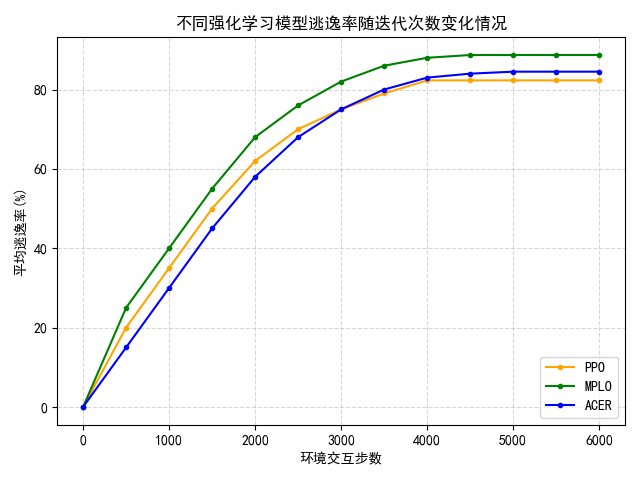
\includegraphics[width=0.75\textwidth]{figures/5.1}
	% \caption[这里的文字将会显示在 listoffigure 中]{这里的文字将会显示在正文中}
	\caption{Training Performance Comparison among Different RL Models}\label{fig:5.1}
\end{figure}

In the modification cost aspect, MPLO are also comparative. Its average perturbation time is 3.8, slightly higher than 3.2 of PPO, extremely lower than 4.1 of ACER, indicating that MPLO can complete the goal with lower operation steps at the premise that different models generate same amount adversarial samples, reducing original file structure disruption, improving the generated samples' concealment and functional retention.

Considering the convergence speed, MPLO achieves policy convergence at 4,500 steps, slower than 4,200 steps of PPO but faster than 5,000 steps of ACER, reflecting that MPLO gets an effective balance between exploration and exploitation. Through multi-dimensional strategy evaluation mechanisms, it can maintain the balance between exploration and exploitation, rapidly approaching optimal disturbance strategies without requiring excess sample replay and exceeding training iterations.

\begin{table}[htbp]
	\centering
	\caption{Performance Comparison between Different RL Models}
	\label{tab:5.9}
	\begin{tabular*}{0.9\textwidth}{@{\extracolsep{\fill}}cccc}
		\toprule
		Model & Average Evasion Rate & Average Perturbation Steps & Convergence Speed(Environment Interaction Steps) \\
		\midrule
		PPO & 82.3\% & 3.2 & 4200 \\
		MPLO & 88.7\% & 3.8 & 4500 \\
		ACER & 84.5\% & 4.1 & 5000 \\
		\bottomrule
	\end{tabular*}
\end{table}

\section{Comparison With Other Adversarial Sample Generation Models}

To comprehensively certify MPLO's effectiveness in adversarial sample generation, this research selects MalConv\cite{raff2017malware} as the target detection model, analyzing its evasion attack performance and the other RL model's performance in the same experiment environment. The comparative experiment follows the unified setting standard, adopting 1,000 malicious ELF files as the attack target and restraining the maximum modification step to 20 to ensure the fairness and comparability of the experiments.

To evaluate the performance comprehensively, this research conducts quantitative comparative analysis on evasion success rate (the rate of generated adversarial samples that can successfully evade the detection of the target detector), average modification times (the average bytes modified in each successful sample) and average generating time (the time required for each sample generation) respectively. The results are illustrated in Table \ref{tab:5.10}.

\begin{table}[htbp]
	\centering
	\caption{Evasion Rate Comparison of Pervalent Detection Models}
	\label{tab:5.10}
	\begin{tabular*}{0.9\textwidth}{@{\extracolsep{\fill}}cccc}
		\toprule
		Model & Average Evasion Rate & Average Modification Steps & Average Generating Time \\
		\midrule
		Baseline & 48.20\% & 5.4 & 212ms \\
		MPLO & 71.25\% & 4.7 & 186ms \\
		DP-GAN & 67.70\% & -- & -- \\
		\bottomrule
	\end{tabular*}
\end{table}

The comparison between MPLO and DP-GAN shows that MPLO exhibits an obvious advantage. The average evasion rate of MPLO is 71.25\%, which is significantly higher than DP-GAN's 67.70\%, represents that MPLO has a higher success rate in adversarial sample generation.

Meanwhile, the average modification times of MPLO decreases to 4.7, which is lower than Baseline's 5.4, indicating that its perturbations are more compact, achieving evasion in less operation steps, thus retaining original sample's semantics and functionality more effectively.

In the evaluation of generation efficiency, the average generation time of MPLO is 186ms, 12\% faster than Baseline's 212ms. This performance development further verifies that MPLO exhibits higher practicality and deployment advantages in scenarios with large-scale samples and high evasion requirements.

To evaluate the dynamic evasion capability in real environments of the adversarial sample generation framework proposed in this research, this research uploads parts of generated samples to Tencent Habo dynamic analysis platform to conduct behavioral analysis detection. Tencent Habo is one of the sandbox analysis platforms that is widely used with multiple engines dynamic detection. It can simulate executing samples in real systems and record suspicious behavioral features, such as file operations, process calls, registry modifications and network connections.

In this research, DDoS Trojan samples are selected as representatives. The platform returns detection scores and behavioral labels after the samples are uploaded to Tencent Habo. The result demonstrates that the results of samples processed by adversarial strategies changes from malicious to unknown.

\begin{figure}[hbt]
	\centering
	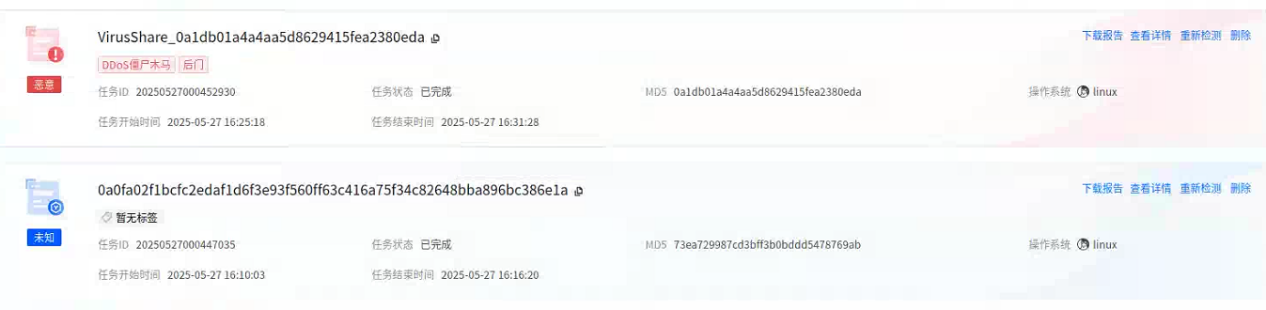
\includegraphics[width=0.75\textwidth]{figures/5.2}
	% \caption[这里的文字将会显示在 listoffigure 中]{这里的文字将会显示在正文中}
	\caption{Comparison of Habo Detection Results before and after Processing}\label{fig:5.2}
\end{figure}

Besides, suspicious behaviors (e.g., remote thread injections, suspicious network communications, memory shellcode execution) were significantly reduced or undetected.
%This confirms that generated samples evade both static feature matching and dynamic behavioral analysis.

In summary, Tencent Harbo dynamic detection experiment further validates the concealment and validity of multi-disturbance strategies issued in this research, proving that this framework is practically potential and exhibits high research value. 

\section{The Influence of Different Disturbance Combination on Evasion Rate and Generating Efficiency}

To evaluate the necessity of the multi-dimensional adversarial sample generation approach proposed in this research, ablation experiments were designed to test the individual effects of structural, instructional, and behavioral perturbations in the evading malware detection aspect. Each disturbance method was systematically ablated by removing it, allowing analyzing its impact on detection evasion capabilities.

In this experiment, 1,000 randomly selected samples from the malware dataset were perturbed individually using three distinct methods, evaluating performance against the random forest detector trained in this study. Comparison with the baseline group allowed researchers to systematically assess each perturbation's contribution to evasion.

\begin{enumerate}

\item Experimental Group 1: Structural Perturbation

This group adopted structural perturbations by modifying program structures of malware samples (e.g., altering section tables, symbol tables, or rearranging code segments). This method's target is disrupting structural information, preventing static analysis tools from accurately identifying malicious behaviors.

\item Experimental Group 2: Instructional Perturbation

This group solely employed instructional perturbations by modifying, reordering, or replacing instructions in malware samples. Modification examples include replacing instructions with functional equivalents or rearranging execution sequences while preserving program logic unchanged to evade analysis at the instruction level.

\item Experimental Group 3: Behavioral Perturbation

This group exclusively implemented behavioral perturbations through altering malicious behavioral logic. Common techniques included inserting time delays or control-flow obfuscation to delay or modify malicious behavior triggers, thus evading dynamic behavioral analysis.

\item Experimental Group 4: Baseline Group

This group applied the proposed multi-dimensional perturbation method, jointly employing structural, instructional, and behavioral perturbations.
\end{enumerate}

Experimental results are descirbed in Table \ref{tab:5.11}.

\begin{table}[htbp]
	\centering
	\caption{Ablation Experiment Performance Comparison}
	\label{tab:5.11}
	\begin{tabular*}{0.9\textwidth}{@{\extracolsep{\fill}}ccc}
		\toprule
		Perturbation Method & Average Evasion Rate & Average Generating Time \\
		\midrule
		Structural Perturbation & 72.5\% & 156ms \\
		Instructional Perturbation & 52.6\% & 218ms \\
		Behavioral Perturbation & 12.1\% & 175ms \\
		MPLO & 87.2\% & 183ms \\
		\bottomrule
	\end{tabular*}
\end{table}

Comparison with three single disturbance strategies, MPLO comprehensively introduces structural, instructional, and behavioral perturbation mechanisms, achieves the highest evasion rate (87.2\%) and limits the generation time in 183ms. This result exhibits complementary advantages: structural perturbation confuses static features, instructional perturbation enhances fine-grained stealth, and behavioral perturbation enables dynamic evasion. Combining these strategies, it bypasses multi-layered detection defenses for more robust adversarial sample generation with higher adaptivity and stability.

The ablation study confirms both independent and synergistic value of each perturbation strategy in MPLO. Individual strategies show partial evasion capabilities but cannot keep stable while facing multiple detection models.Integrating perturbation strategies in a unified framework significantly enhances overall evasion performance, practical applicability, and robustness against diverse detection models.  

\section{The Influence of Different Disturbance Combination on Functional Integrity}

In adversarial malware sample generation tasks, preserving the original functionality of perturbed samples serves as a critical criterion for evaluating their effectiveness and practical values. Samples that evade detection but lose their malicious functionality diminish their value in real attack scenario simulations, security assessments, and system defense training. Therefore, this study systematically conducts the research on the malicious functionality impact of the three proposed perturbation methods—structural, instructional and behavioral.

\begin{enumerate}

\item Functional Preservation Analysis of Structural Perturbation

Structural perturbation primarily modifies metadata and file structures of programs, such as section table rearrangement, symbol table modification, section addition and section renaming. Such disturbances do not alter the program's instruction logic or execution flow, theoretically maintaining its functional behavior.

Hundreds of structurally perturbed malware samples were executed in the controlled sandbox to observe their crucial behavioral characteristics (e.g., reverse connections, keystroke logging, and file tampering). The results show that most structurally perturbated samples represent highly identical to the original samples. The functionality retention rate reached 92.4\%. The failure samples are mainly caused by disturbing excessively on sections of the loader or disrupting symbol relocation information. These conditions can be fixed by adopting more intricate disturbance controls.

\item Functional Preservation Analysis of Instructional Perturbation

Instructional perturbations aim to modify program code, including equivalent replacement of sequential structures with jumps. These techniques highly depend on following semantic-preserving principles to obfuscate static instruction sequences without altering program logic.

Utilizing Control Flow Integrity (CFI) checks and execution path comparison methods, experimental results demonstrate that more than 96\% of samples maintained original malicious behaviors (e.g., establishing remote communication, data exfiltration) after perturbations and the FRR reached 93.7\%. Minor failure samples occurred due to disrupted jump logic, stack imbalance, or calling convention violations, which suggests that future implementations should incorporate stricter constraints for semantic consistency.

\item Functional Preservation Analysis of Behavioral Perturbation

Behavioral perturbations interfere with behavioral analysis tools by delaying malicious behavior triggers, inserting obfuscated control flows, and introducing conditional execution dependencies. This strategy alters the triggering mechanism rather than the core malicious logic, resulting in conditional functionality preservation.

\end{enumerate}

In this research, prolonging disturbed samples' execution time verifies whether the original malicious behaviors can be triggered. The results show that 98\% of behaviorally perturbed samples fully replicated original malicious behaviors under appropriately configured trigger conditions.

To comprehensively compare functional retention results of three perturbation strategies, this research compile statistics on each sample's success execution rate and functional retention rate. The results are provided in Table \ref{tab:5.12}.

\begin{table}[htb]
	\centering
	\caption{Functional Preservation Research Results}
	\label{tab:5.12}
	\begin{tabular*}{0.9\textwidth}{@{\extracolsep{\fill}}ccc}
		\toprule
		Perturbation Type & Successful Execution Rate(\%) & Functional Preservation Rate(\%) \\
		\midrule
		Structural Perturbation & 99.2 & 92.4 \\
		Instructional Perturbation & 96.5 & 93.7 \\
		Behavioral Perturbation & 82.7 & 98.0 \\
		\bottomrule
	\end{tabular*}
\end{table}

All in all, structural perturbation maintains high functionality retention without disrupting program logic. Instructional perturbation achieves strong consistency under controlled constraints. Behavioral perturbation, despite lower execution success rates due to complex triggering mechanisms, exhibits the highest functionality retention capability.

\section{Sample Transferability Analysis}

This research selects representative samples from adversarial samples modified by structural perturbations, instructional perturbations, and behavioral perturbations, and compares them with original malicious samples without modification. All samples were uploaded to VirusTotal for static and dynamic scanning. Detection results from each engine were recorded. The number of engines detecting each sample (i.e., "hit rate") was collected as the metric for evasion capability.

\begin{figure}[htbp]
	\centering
	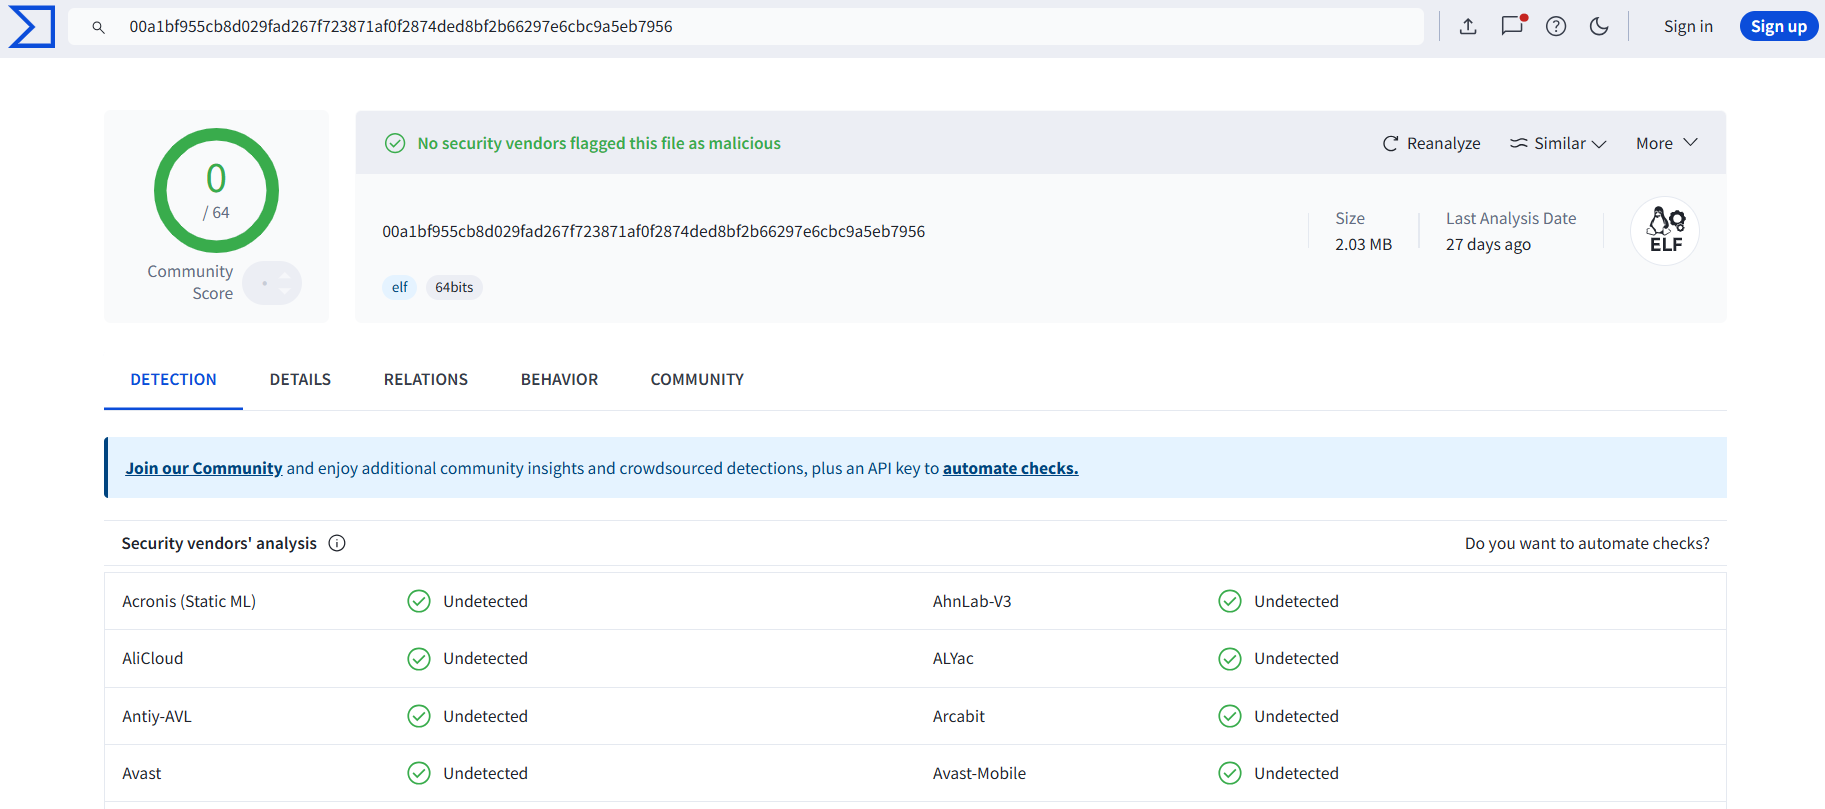
\includegraphics[width=0.75\textwidth]{figures/5.3}
	% \caption[这里的文字将会显示在 listoffigure 中]{这里的文字将会显示在正文中}
	\caption{VirusTotal Scanning Results After Adversarial Learning}\label{fig:5.3}
\end{figure}


To better illustrate the evasion effect, the VirusTotal detection rate $v_t$ is defined as the ratio of antivirus engines detecting maliciousness to the total number of engines, calculated as the formulation below:
\begin{equation}
v_t = \frac{D_e}{A_e}
\tag{5.9}
\end{equation}

$D_e$ is the number of antivirus engines detecting maliciousness, while $A_e$ presents the total number of antivirus engines.

Table \ref{tab:5.13} lists the detection rates $v_{t1}$ before evasion, $v_{t2}$ after evasion, and the decline rate $vt_{down}$ of20 samples on VirusTotal.

\begin{table}[htbp]
	\centering
	\caption{Comparison of VirusTotal Scanning Results before and after Processing}
	\label{tab:5.13}
	\begin{tabular*}{0.9\textwidth}{@{\extracolsep{\fill}}cccc}
		\toprule
		Name & Detection Rate Before Process & Detection Rate After Process & Decline \\
		\midrule
		e601de9bb0828bae5eec828547d18e84 & 39/62 & 2/62 & 94.87\% \\
		e61865927c25a33f57b3385f59d45bf8 & 40/59 & 3/62 & 92.5\% \\
		e62288919ce96bbe2d382c49797d5e99 & 41/62 & 5/62 & 87.8\% \\
		e6344bb726c1b97e277c478bb7a2ddab & 32/61 & 3/60 & 90.62\% \\
		e6450e7a705060df1795b18bc853416d & 40/62 & 2/62 & 95.0\% \\
		e64e06c16591f46ec8759be807f7b34c & 38/62 & 0/62 & 100.00\% \\
		e69ba88b83c142b2f04f857787fdfb5e & 38/62 & 3/62 & 92.11\% \\
		e6df850bfa010aa039511504ccd917db & 37/62 & 5/62 & 86.49\% \\
		e6e6891c01c56533919a3f9f677f6467 & 41/62 & 2/62 & 95.12\% \\
		026f98e26942d5745b589069cf6dd143 & 41/62 & 3/62 & 92.68\% \\
		e704b5769c02ff5ccc7f53ca46d63fd2 & 43/61 & 4/62 & 90.70\% \\
		e711723f3301251615d6009382c7234b & 43/62 & 3/62 & 93.02\% \\
		056e32863c0483922464fee50b2bbd37 & 39/62 & 2/62 & 94.87\% \\
		031be2bf69f1fbe13d78c2ac93508753 & 41/62 & 3/62 & 92.68\% \\
		e789b8bb45c88a64f682fb434eb50bcc & 38/62 & 2/62 & 94.74\% \\
		e9ea5cbcba4f9406f9926ff0080997a3 & 42/62 & 5/62 & 88.10\% \\
		e9ee698553866065fa6bdb0764df2564 & 37/62 & 4/62 & 89.19\% \\
		eacd3c9972ab6c22267d3eda9addf9a6 & 40/61 & 0/62 & 100.00\% \\
		032de9e9ee32b91053b8195422fb2133 & 41/62 & 3/62 & 92.68\% \\
		eaf1a8c6eb5fa1641517de35fefb1a18 & 36/63 & 5/62 & 86.11\% \\
		\bottomrule
	\end{tabular*}
\end{table}

Experimental results indicate that adversarial samples processed by perturbation exhibit extremely lower overall detection rates on VirusTotal than original samples, exhibiting strong transferability. Structural perturbations achieved the most stable evasion, with multiple static analysis-dependent engines failing to identify malicious features. Instructional perturbations showed limited evasion across engines, yielding relatively overall smaller variations. Behavioral perturbations effectively evaded engines with weaker dynamic detection capabilities, but there still exist partial detections in engines supporting sandbox analysis. The limitation shows platform-specific dependencies in dynamic feature interference.

Furthermore, different perturbation methods affected engine types distinctly. Structural perturbation primarily disrupted engines relying on static structure parsing and feature extraction. Instructional perturbation impacted detectors based on instructional signatures or machine learning models. Behavioral perturbation more readily evaded dynamic mechanisms based on sandbox execution paths and behavioral patterns. These results further validate the adaptability and practical utility of adversarial perturbations in multi-engine, cross-platform detection environments.


